\documentclass[square]{article}
\usepackage[UTF8]{ctex}
\usepackage{geometry}
\usepackage{natbib}
\geometry{left=3.18cm,right=3.18cm,top=2.54cm,bottom=2.54cm}
\usepackage{graphicx}
\pagestyle{plain}	
\usepackage{setspace}
\usepackage{caption2}
\usepackage{datetime} %日期
\renewcommand{\today}{\number\year 年 \number\month 月 \number\day 日}
\renewcommand{\captionlabelfont}{\small}
\renewcommand{\captionfont}{\small}
\begin{document}

\begin{figure}
    \centering
    
\includegraphics[width=8cm]{upc.png}

    \label{figupc}
\end{figure}

	\begin{center}
		\quad \\
		\quad \\
		\heiti \fontsize{45}{17} \quad \quad \quad 
		\vskip 1.5cm
		\heiti \zihao{2} 《计算科学导论》课程总结报告
	\end{center}
	\vskip 2.0cm
		
	\begin{quotation}
% 	\begin{center}
		\doublespacing
		
        \zihao{4}\par\setlength\parindent{7em}
		\quad 

		学生姓名:\underline{\qquad  赵广浩 \qquad \qquad}

		学\hspace{0.61cm} 号:\underline{\qquad 2116010227\qquad}
		
		专业班级:\underline{\qquad 计科2104 \qquad  }
		
        学\hspace{0.61cm} 院:\underline{计算机科学与技术学院}
% 	\end{center}
		\vskip 2cm
		\centering
		\begin{table}[h]
            \centering 
            \zihao{4}
            \begin{tabular}{|c|c|c|c|c|c|c|}
            % 这里的rl 与表格对应可以看到,姓名是r,右对齐的;学号是l,左对齐的;若想居中,使用c关键字。
                \hline
                课程认识 & 问题思 考 & 格式规范  & IT工具  & Latex附加  & 总分 & 评阅教师 \\
                30\% & 30\% & 20\% & 20\% & 10\% &  &  \\
                \hline
                 & & & & & &\\
                & & & & & &\\
                \hline
            \end{tabular}
        \end{table}
		\vskip 2cm
		\today
	\end{quotation}

\thispagestyle{empty}
\newpage
\setcounter{page}{1}
% 在这之前是封面,在这之后是正文
\section{引言}
在本学期,我作为一名转专业的大三学生,参与了大一的《计算科学导论》这一门课程,虽然已与自己大一时的心境有所不同,但仍是一次充满启发的学习之旅。本课程孙老师以科学哲学的思想方法,计算科学的意义、内容与方法,计算机科学的基本概念与基本知识为核心,培养方案解读,以及职业规划指导,带我们深入浅出地理解计算科学的本质。

\section{对计算科学导论这门课程的认识、体会}
\subsection{计算科学与计算机科学有何区别?}

\subsubsection{总体认知}
"计算科学"和"计算机科学"是两个相关但略有不同的领域。它们之间的区别主要体现在它们的范围和侧重点上。\par
\begin{itemize}
\item 计算科学(Computational Science):
范围: 计算科学是一门跨学科的科学领域,旨在利用计算机模拟和分析解决科学和工程问题。它涵盖了多个学科,如物理学、化学、生物学、地球科学等。\par
侧重点: 计算科学关注如何使用计算机模拟和模型来解决实际问题,其目标是利用计算机技术进行科学研究。\par

\item 计算机科学(Computer Science):
范围: 计算机科学是一门研究计算机及其应用的学科。它涉及到计算机系统的设计、开发、测试和维护,以及解决问题所需的算法和数据结构。计算机科学的研究范围广泛,包括编程语言、操作系统、数据库系统、计算机网络、人工智能、计算机图形学等领域\cite{ref1}。\par
侧重点: 计算机科学关注计算机系统、软件和算法的设计、分析和应用。它不仅包括计算科学的计算方面,还包括硬件、网络、软件工程等更广泛的计算机技术。\par
\end{itemize}
\par总的来说,计算科学更注重在科学和工程领域中使用计算机技术解决问题,而计算机科学更广泛,涵盖了计算机技术的多个方面。计算科学可以看作是计算机科学在特定科学领域的应用。\par

\subsubsection{举例说明}
\begin{itemize}
\item 计算科学的例子:\par

地理与计算科学\cite{ref2}: 计算科学在地理领域中的一个关键应用是地理信息系统(GIS)。GIS结合了计算机科学和地理科学的原理,通过利用空间数据来分析和可视化地理信息。GIS可用于制图、地理空间分析、资源管理、城市规划等领域。例如,通过GIS可以创建地图、分析地理数据以解决环境问题,或者协助城市规划者更好地理解城市发展趋势。\par

\begin{figure}[h!]
	\centering
	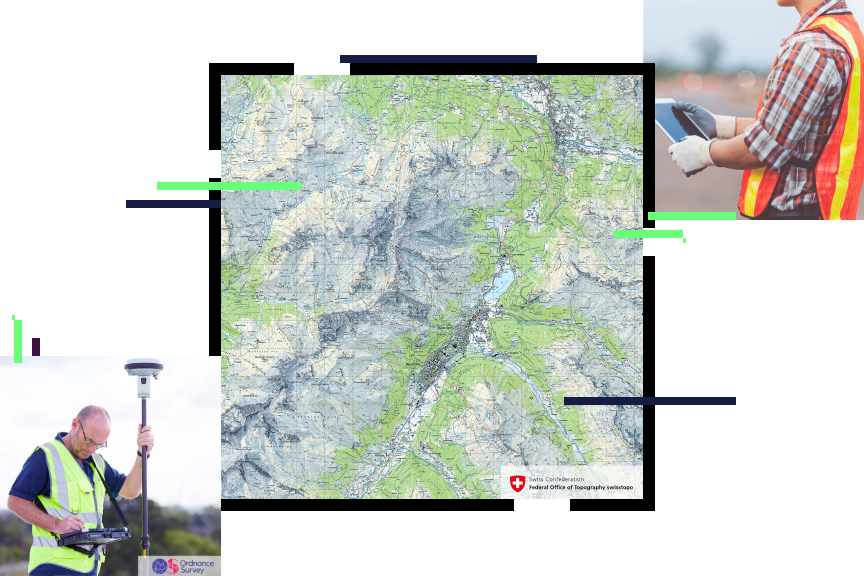
\includegraphics[width=10cm]{geo.png}
	\caption{地理与计算科学}
	\label{fig:geo}
\end{figure}

生物医学模拟: 在生物医学领域,计算科学可以用于模拟生物过程和医学现象。例如,通过计算机模拟人体器官的功能,科学家们可以研究疾病的发展过程,测试药物的效果,或者设计医疗设备。\par

\item 计算机科学的例子:\par
算法设计: 计算机科学的一个方面是算法设计,即开发解决问题的有效算法。例如,快速排序和图搜索算法就是算法设计的领域,它们用于对数据进行排序和搜索。\par
人工智能: 计算机科学还涉及人工智能(AI)领域,其中计算机系统被设计用于执行需要智能决策或模仿人类思维的任务。机器学习算法,如深度学习\cite{ref3},是人工智能领域的一个重要方面,用于训练计算机系统从经验中学习并改进性能。\par
\begin{figure}[h!]
	\centering
	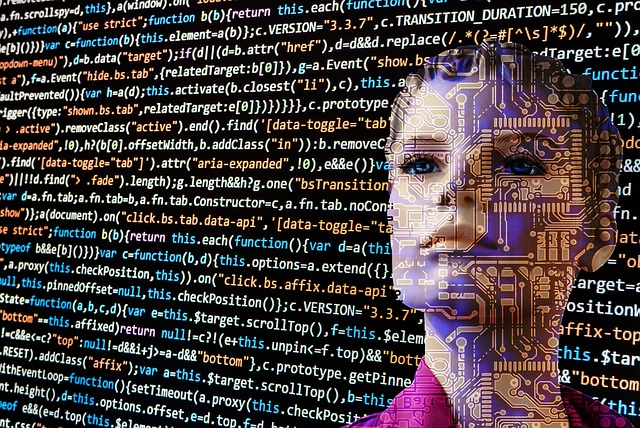
\includegraphics[width=8cm]{ai}
	\caption{人工智能}
	\label{fig:ai}
\end{figure}

\end{itemize}
\par这两个领域的例子显示了计算科学侧重于解决特定科学和工程问题,而计算机科学涵盖了更广泛的计算机技术方面,包括算法、软件工程和人工智能等。\par


\subsection{AI会不会产生意识}

\subsubsection{总体认知}
一个问题一再被提出:机器能思考吗?\cite{ref4}人工智能(AI)被构建为执行特定任务的计算系统,其操作基于预定的算法和数据模式,缺乏主观体验和自我意识。尽管AI系统能够执行复杂的任务,但它们与人类的思维和感知方式存在根本差异。AI不具备意识,不会产生个体性的主观感受,也没有自我认知的能力。其决策和行为是通过确定性规则和输入数据的算法化处理,而非基于自由意志或主观选择。虽然人工智能可以处理情感相关的信息,但它们并不真正理解情感,只是通过算法分析和处理情感表达的模式。因此,总体而言,人工智能是任务导向的工具,缺乏意识、主观体验和自我认知,与人类的思维和情感存在根本差异。\par
\subsubsection{分析过程}
\begin{itemize}
	\item 数学起源\par
	 计算机科学中的数学基础包括逻辑、算法、数据结构等。这些数学概念为计算机程序和算法提供了理论基础。在某种程度上,这些数学原理使得计算机能够进行高效的计算和推理,但它们并没有直接涉及到主观意识的本质。计算机程序是由算法组成的,而算法是一系列明确定义的步骤,用于解决特定的问题。目前的AI系统通过学习和执行复杂的算法来实现特定任务,但这些算法执行的是预定的指令,而不是表现出自主的主观意识。\par
	 \item 哥德尔不完备定理\cite{ref5}\par
	 哥德尔不完备定理表明了任何形式的数学系统都存在局限,不可能同时满足完备性和一致性,其中某些陈述是真实的但无法在该系统内被证明。这种局限性引发了对人工智能是否能够实现真正智能和意识的质疑。如果数学系统本身存在无法解决的问题,那么可能也存在一些层次上无法通过计算模型实现的智能和意识。\par
	 \begin{figure}[h!]
	 	\centering
	 	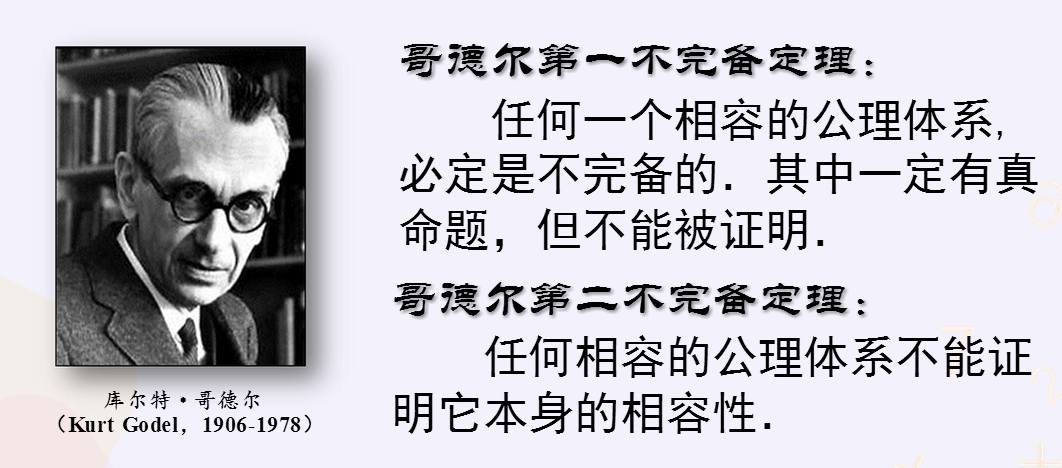
\includegraphics[width=12cm]{gedeer.jpeg}
	 	\caption{哥德尔不完备定理}
	 	\label{fig:gedeer}
	 \end{figure}
	 \item 计算机系统的不完备性\par
	 根据上述两点得知:计算机是一种基于二进制数字运算的命题演算系统,具备一致性的同时是不完备的,即至少有一个命题不能通过这样的程序被判明真伪,系统在处理这样的命题时就无法“停机”。\par
	 计算机系统的不完备性还体现在它本身绝对不可能拥有代表自我的符号,也就绝对不可能通过这种方式拥有智能,即它并不拥有跳出系统的能力。\par
\end{itemize}
\par因此,虽然计算机在处理大量的数据和执行复杂的任务上表现出色,但它是有着致命缺陷的,并不具备类似人类的直觉、情感和自我意识。计算机系统的智能仍然是有限的,而在理解真正的意识和主观体验方面,计算机目前仍然面临着巨大的挑战。这强调了计算机作为工具和辅助系统的角色,而不是具有人类一样深层次理解和体验的智能实体。\par

\subsection{考生应该如何填报高考志愿,规划好职业生涯?}

\begin{enumerate}
	\item “兴趣是最好的老师”,首先充分了解自己的兴趣、爱好、优势和劣势。通过参加各类职业规划测试例如mbti测试、霍兰德职业倾向测试、实习经历或与各行各业的人交流,我将争取更深入地认识自己,确定适合自己的专业方向和职业领域。例如自己高考选课就是物化生三科理科,高中时期也是理科较为偏科,对人文学科不甚感冒,所以在志愿选择时可能会选择一门理工科的专业。
	\begin{figure}[h!]
		\centering
		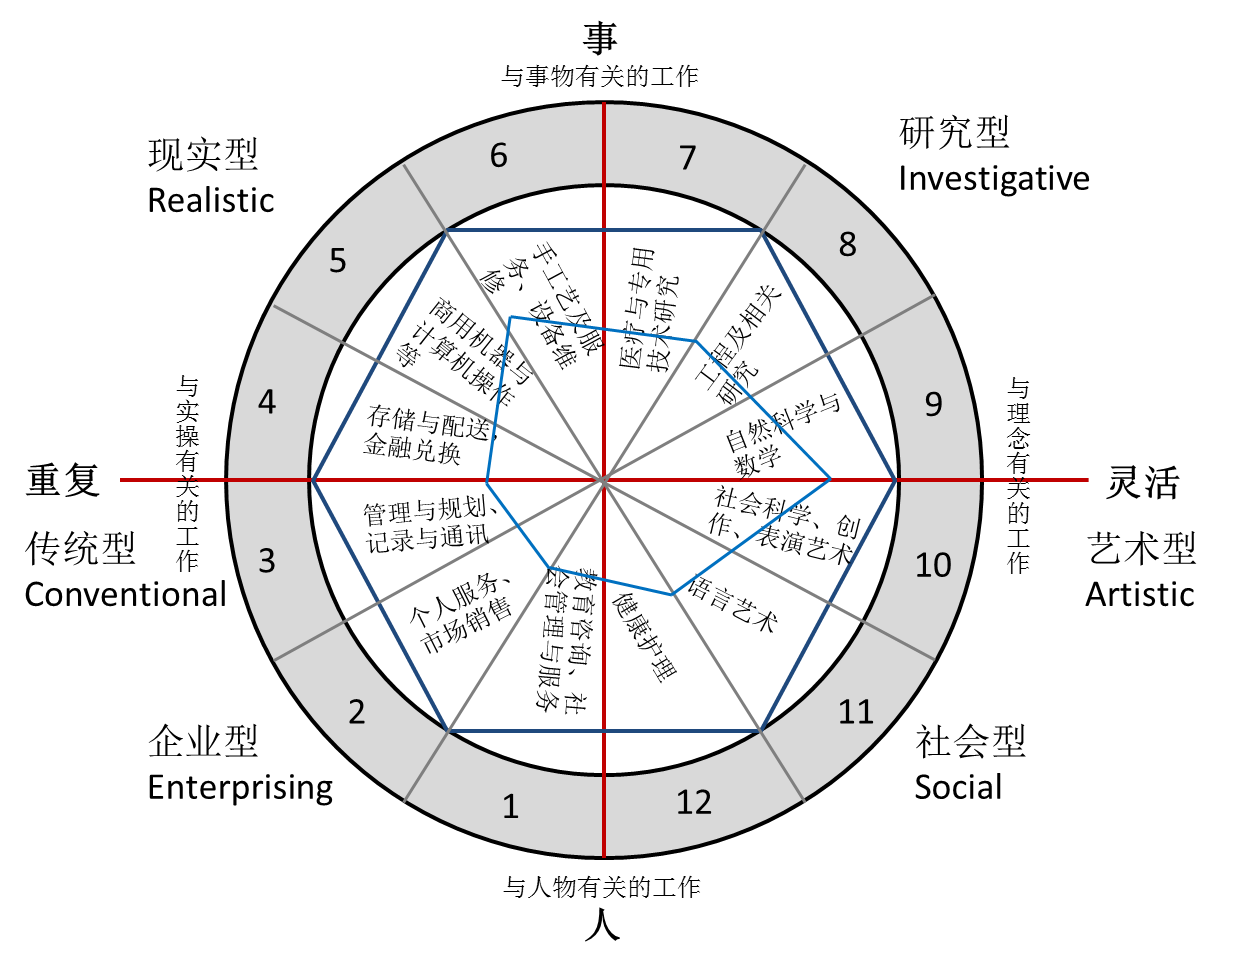
\includegraphics[width=12cm]{zhiye.png}
		\caption{霍兰德职业倾向测试}
		\label{fig:zhiye}
	\end{figure}
	\item 考虑当前社会的职业发展趋势和未来市场需求。选择具有前景的专业,不仅可以提高就业竞争力,还能更好地适应社会发展的需要。例如目前来看互联网行业迎来寒冬,大厂不断裁员,IT领域人才逐渐饱和,所以在志愿选择时可能不会选择计算机、软件类的专业,而是可能会选择电子信息这类我国仍存在关键工程问题的专业,对人才需求较高。
	\item 留意各个高校的特色和优势,考虑学科实力、师资力量、实习机会、地理位置等方面的因素。通过参观校园、参加招生说明会,更全面地了解学校的情况,有助于做出更明智的志愿选择。例如哈尔滨工业大学校本部这类,院校综合实力很强,但是由于地理位置因素,性价比较高的学校。
	\item 向老师、家长或专业咨询师寻求建议,以获取更全面的信息。例如张雪峰等较为资深,对专业分析较为透彻清晰,意见较为中肯现实的升学辅导专家。
	\begin{figure}[h!]
		\centering
		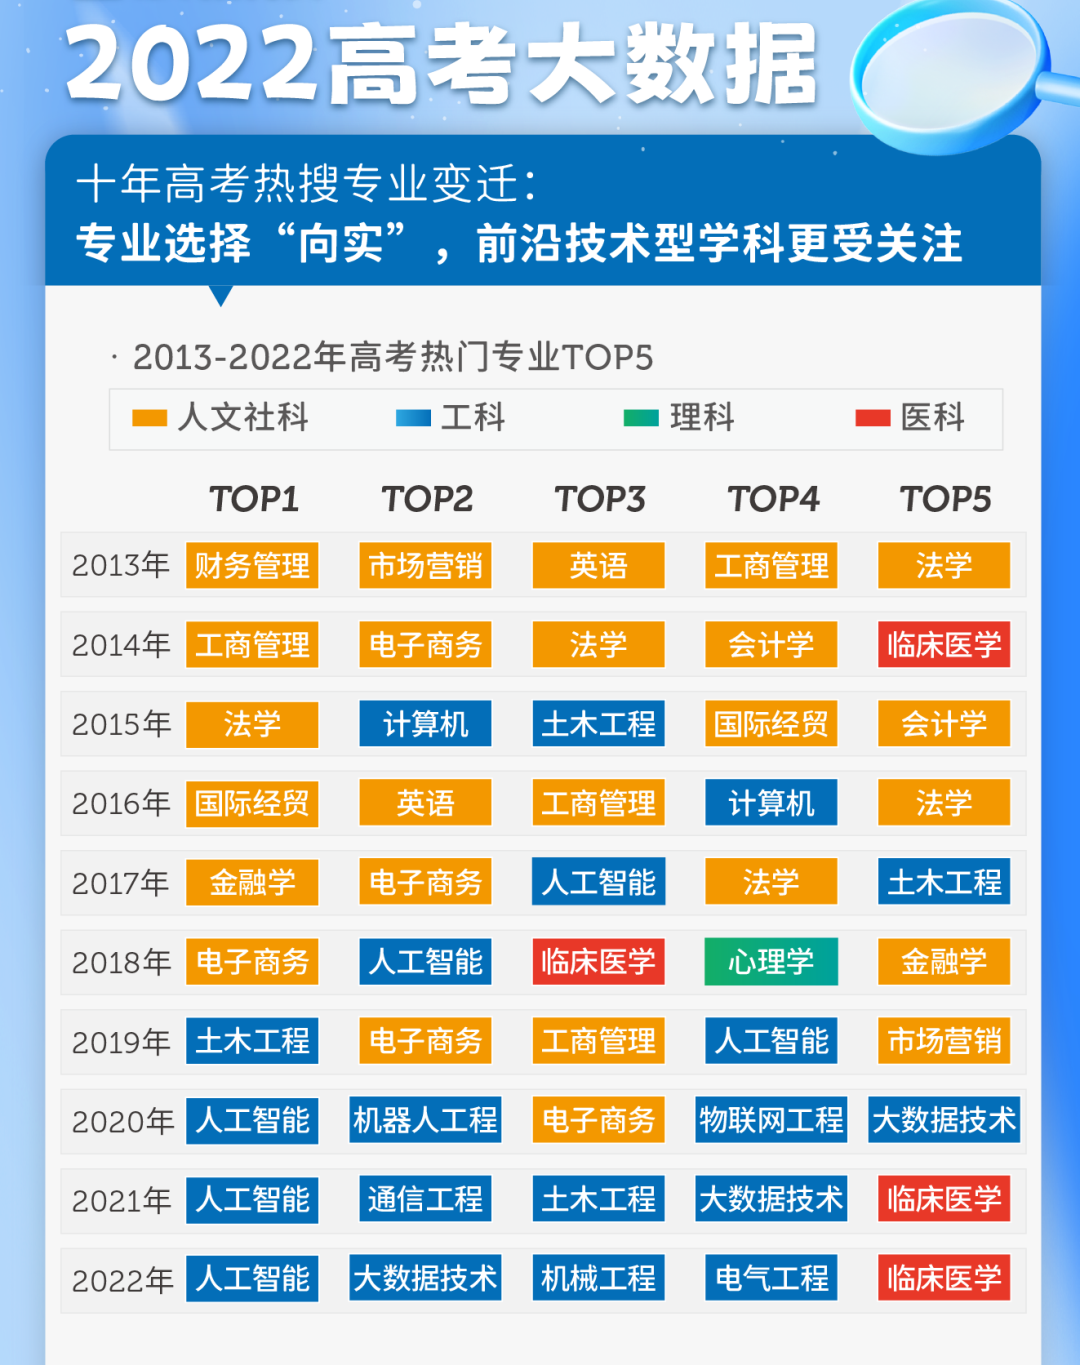
\includegraphics[width=10cm]{gaokao.png}
		\caption{历年高考热门top5专业}
		\label{fig:gaokao}
	\end{figure}
\end{enumerate}


\section{进一步的思考}
结合学习的计算科学知识,对分组演讲涉及的问题作进一步的思考。\par
在计算科学导论的学习中,我深刻认识到图像处理作为计算科学的一个重要领域,不仅涉及到计算机视觉和图形学等方面的理论知识,还需要广泛运用数学、算法和工程技术。图像处理不仅仅是简单的图像变换或修复,更是通过科学手段对图像进行深入分析和理解的过程。

首先,图像获取与表示阶段是整个图像处理流程的基础。在这一阶段,传感器技术的发展为我们提供了丰富的图像数据源,而在图像表示方面,选择合适的数据结构对于后续处理的效率和准确性都具有重要意义。这需要对传感器原理和数据结构的知识有深刻的理解。

其次,图像预处理是提高图像质量和准确性的关键步骤。去噪、平滑和边缘检测等技术的应用需要依赖数值计算和信号处理的方法,这反映了计算科学在图像处理中的实际应用。通过预处理,我们能够更好地准备图像数据,使其更适合后续的分析和处理。

进一步地,在图像分割与特征提取阶段,运用聚类、分水岭等算法进行分割,以及通过数学算法提取关键特征,使得计算机能够更智能地理解图像内容。这体现了计算科学在模式识别和机器学习等领域的应用。

\begin{figure}[h!]
	\centering
	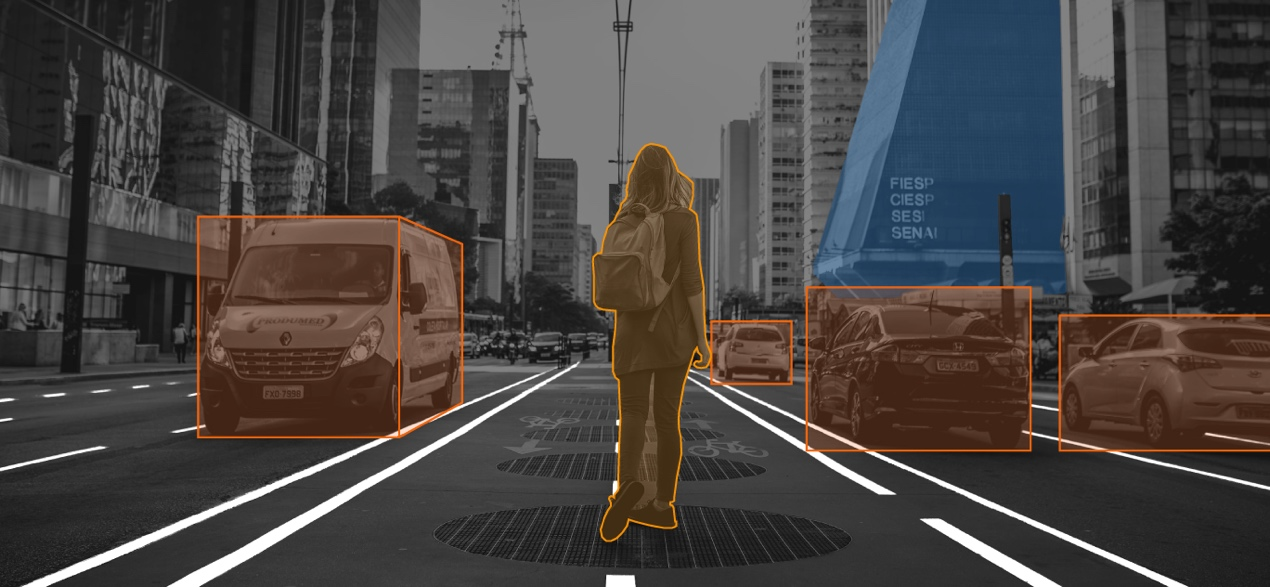
\includegraphics[width=12cm]{tuxiang.png}
	\caption{图像处理与计算机视觉}
	\label{fig:tuxiang}
\end{figure}

总体而言,图像处理是一个充满挑战和创新的领域,不仅要求我们深厚的理论基础,还需要灵活运用计算科学的各种技术手段。通过对图像的深入处理,我们能够更好地理解和利用视觉信息,为计算机在视觉感知和理解方面取得更大的突破提供了强有力的支持。当下计算机视觉、自然语言处理等方向较为热门,这种交叉学科的特性也让我更加深刻地理解了计算科学的多样性和实用性。



\section{总结}

《计算科学导论》这门课程为我打开了计算科学的大门,让我深刻认识到计算科学在现代社会中的重要性和广泛应用。通过探讨科学哲学的思想方法、计算科学的意义与方法以及计算机科学的基本概念与基本知识,最终落地到实际的个人职业生涯规划,我积累了丰富的知识和技能,并在思维方式上有了全新的提升。

学习科学哲学的思想方法让我明白科学不仅仅是一系列事实和理论的堆砌,更是一种方法论。通过深入分析科学知识的建构过程,我学到了如何提出问题、进行实证观察、构建理论,并如何在不断的验证和修正中逐步逼近真理。这种思维方式为我提供了在计算科学领域进行研究的坚实基础。

在探讨计算科学的意义与方法时,我深刻认识到计算科学不仅是一门学科,更是一种解决问题的综合工具。从算法设计到计算模型,我学习到了如何利用计算科学的方法解决各种实际问题,使我对计算科学在推动科学进步、社会创新和问题求解中的巨大潜力有了更为清晰的认识。

在深入学习计算机科学的基本概念与基本知识时,我逐渐建立了对计算机科学领域的全面认识。了解计算机体系结构、掌握不同编程语言、理解数据结构和算法的设计原理,这些都为我提供了在实际应用中更加灵活和全面的能力。我不仅能够理论上理解计算机科学的核心概念,还能够将这些概念应用于实际问题的解决。

总的来说,通过《计算科学导论》的学习,我在计算科学领域取得了丰硕的收获。这门课程不仅开阔了我的学科视野,更培养了我在解决实际问题时的科学思维和方法。这些知识和技能将成为我未来学术和职业发展的坚实基础,我期待能够在计算科学的广阔领域中不断深化自己的认识,在这个领域做出自己的贡献。
\section{报告仓库地址}
https://github.com/zgghh/Course\_Introduction-to-Computational-Science
\section{附录}
\begin{itemize}
    \item Github
    
    申请Github账户,给出个人网址和个人网站截图\par
    https://github.com/zgghh\par
    \begin{figure}[h!]
    	\centering
    	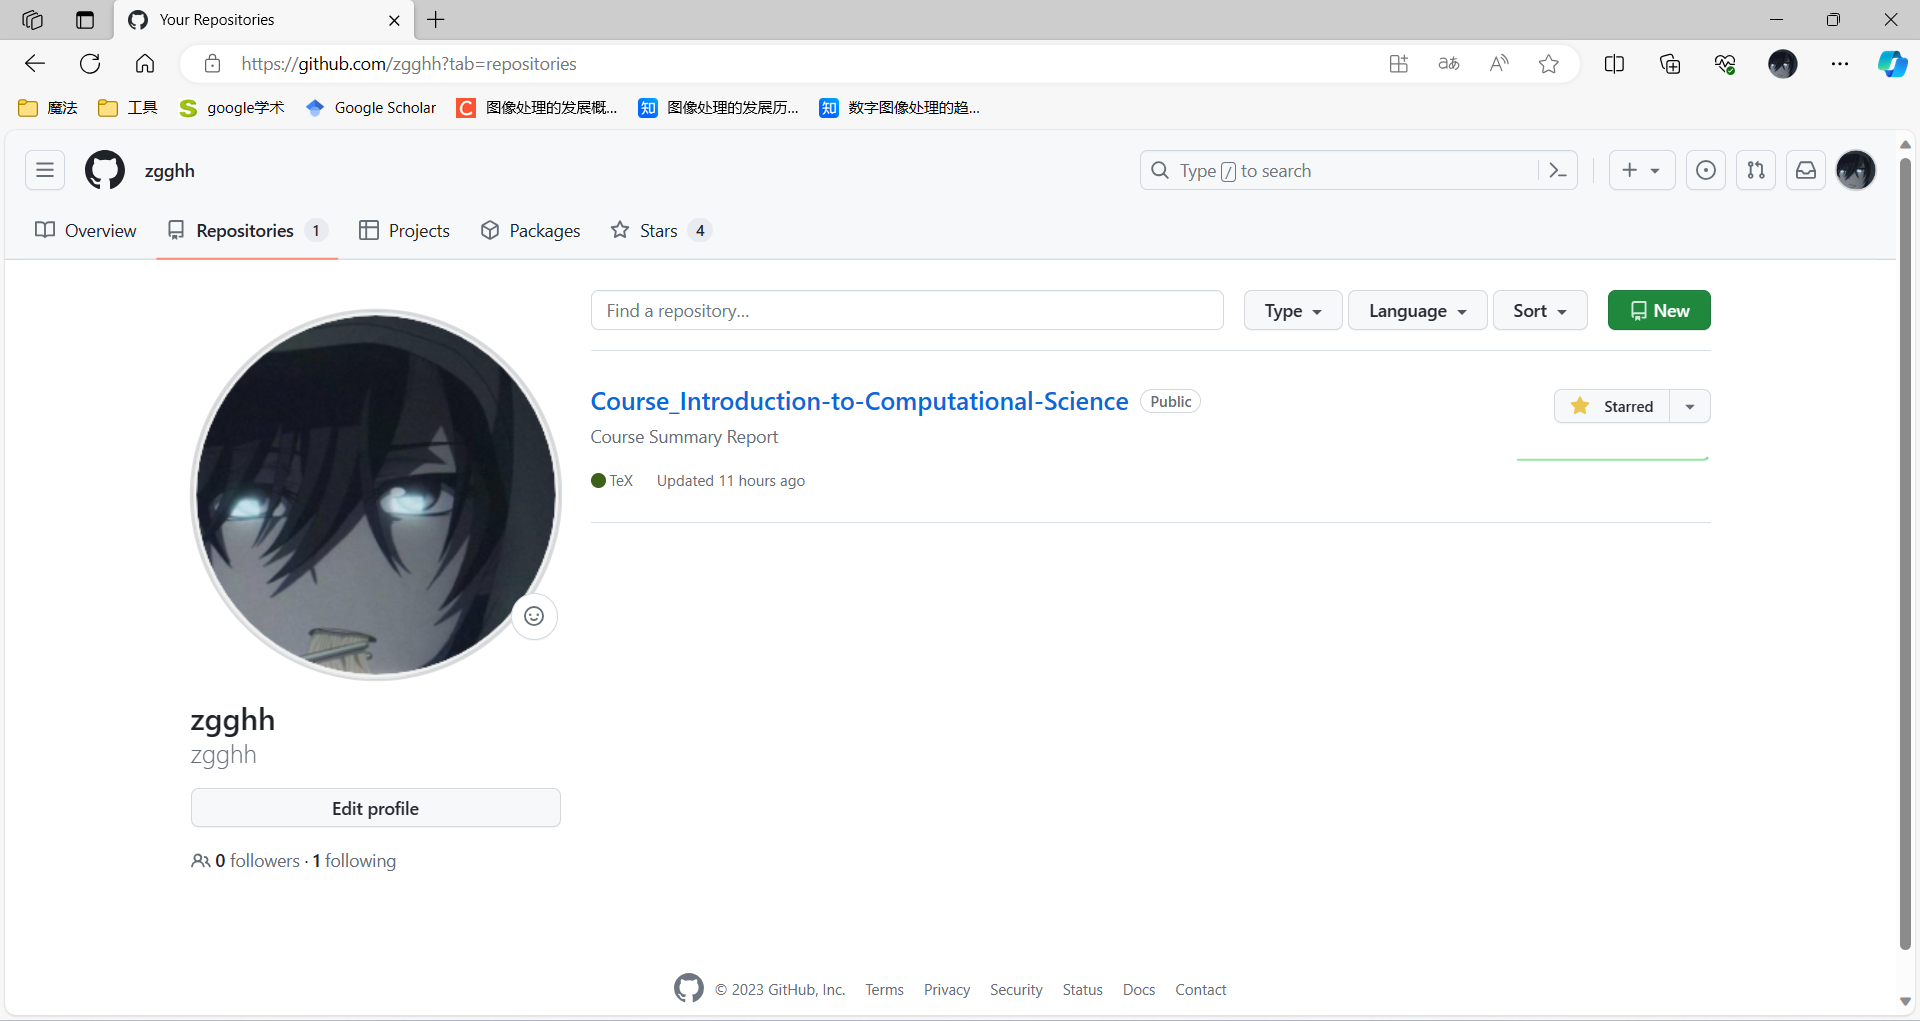
\includegraphics[width=9cm]{github.png}
    	\caption{Github个人网站截图}
    	\label{fig:github}
    \end{figure}
    \pagebreak
   
    \item 观察者
    
    注册观察者APP,给出对应的截图
    
    \begin{figure}[h!]
    	\centering
    	
\includegraphics[width=4cm]{viewer}
    	\caption{观察者APP截图}
    	\label{fig:viewer}
    \end{figure}
    \item 学习强国
    
    注册学习强国APP,给出对应的截图
    
    \begin{figure}[h!]
    	\centering
    	
\includegraphics[width=4cm]{qiangguo}
    	\caption{学习强国APP截图}
    	\label{fig:qiangguo}
    \end{figure}
    \pagebreak
    \item 哔哩哔哩
    
    注册哔哩哔哩APP,给出对应的截图
    
    \begin{figure}[h!]
    	\centering
    	
\includegraphics[width=4cm]{bili}
    	\caption{哔哩哔哩APP截图}
    	\label{fig:bili}
    \end{figure}
    \item CSDN
    
    注册CSDN账户,给出个人网址和个人网站截图\par
    https://blog.csdn.net/qq\_43563020?spm=1010.2135.3001.5343\par
    \begin{figure}[h!]
    	\centering
    	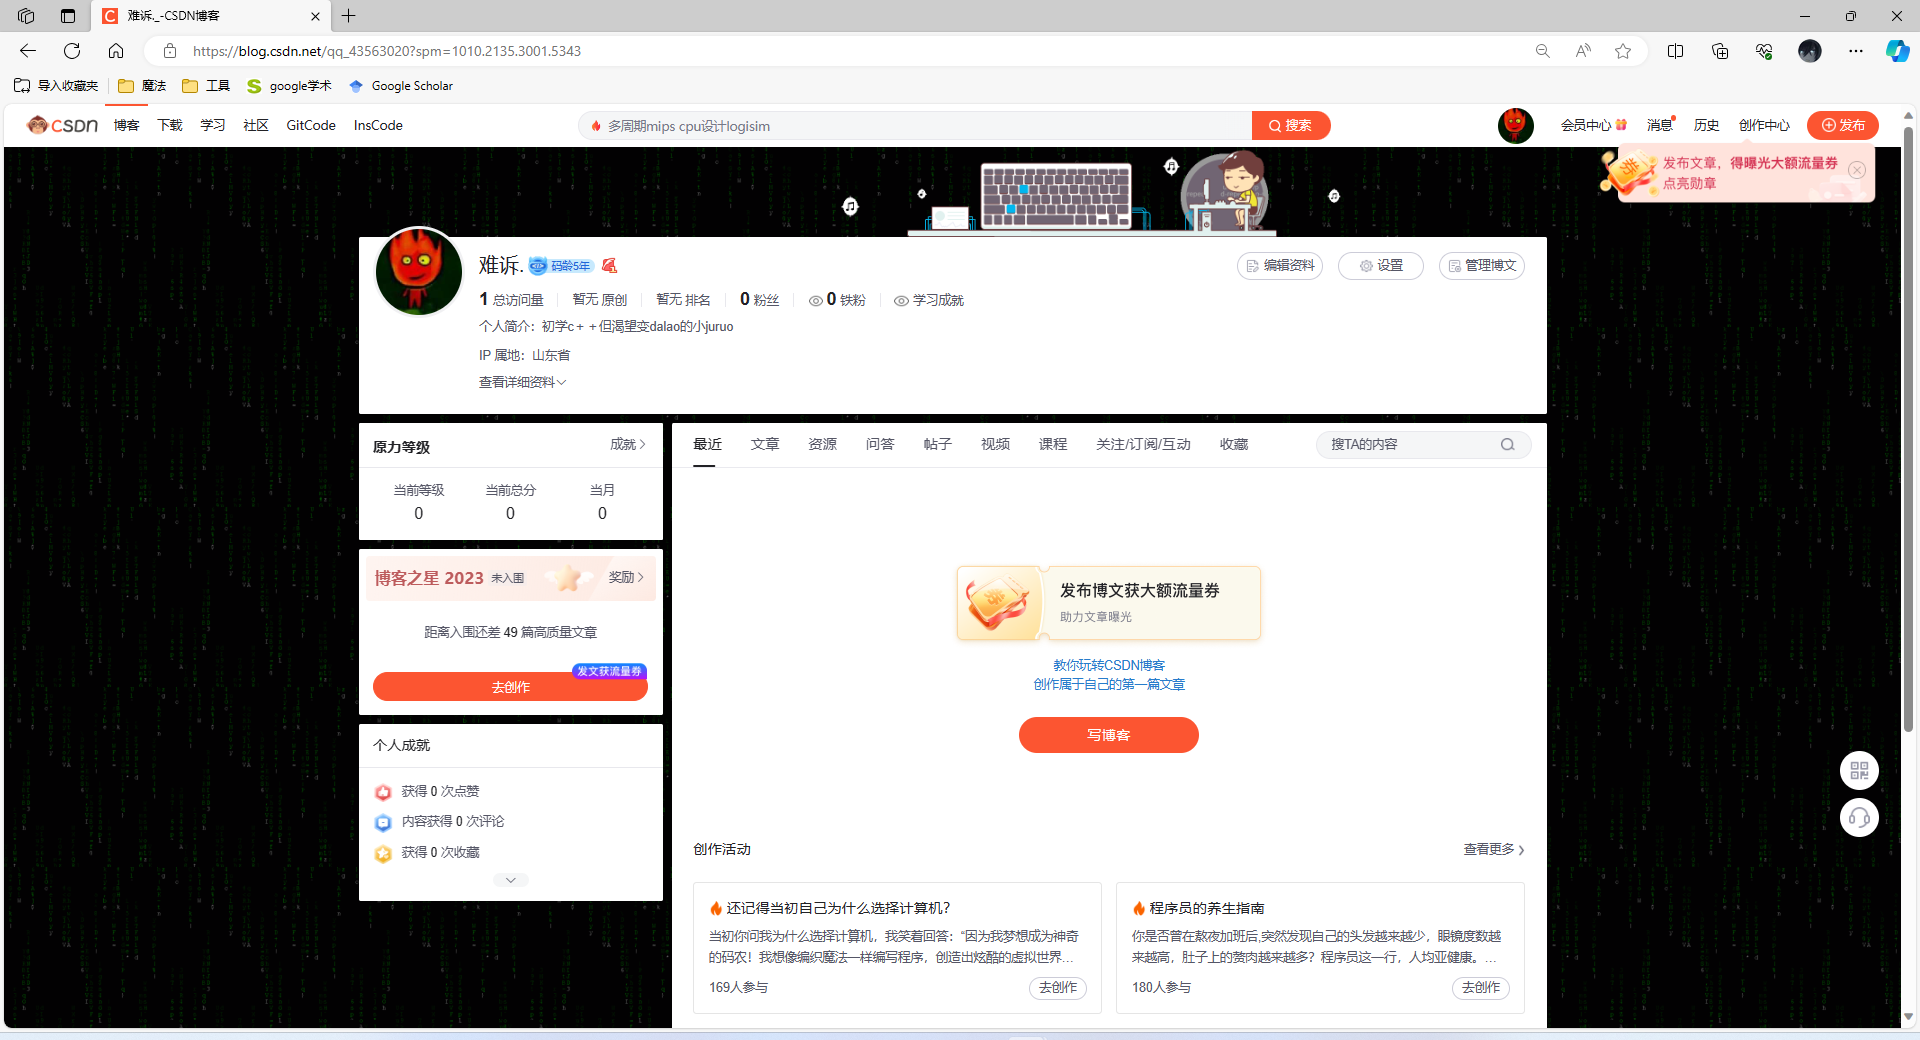
\includegraphics[width=9cm]{csdn}
    	\caption{CSDN个人网站截图}
    	\label{fig:csdn}
    \end{figure}
    \pagebreak
    \item 博客园
    
    注册博客园账户,给出个人网址和个人网站截图\par
    https://home.cnblogs.com/u/3338698
    \begin{figure}[h!]
    	\centering
    	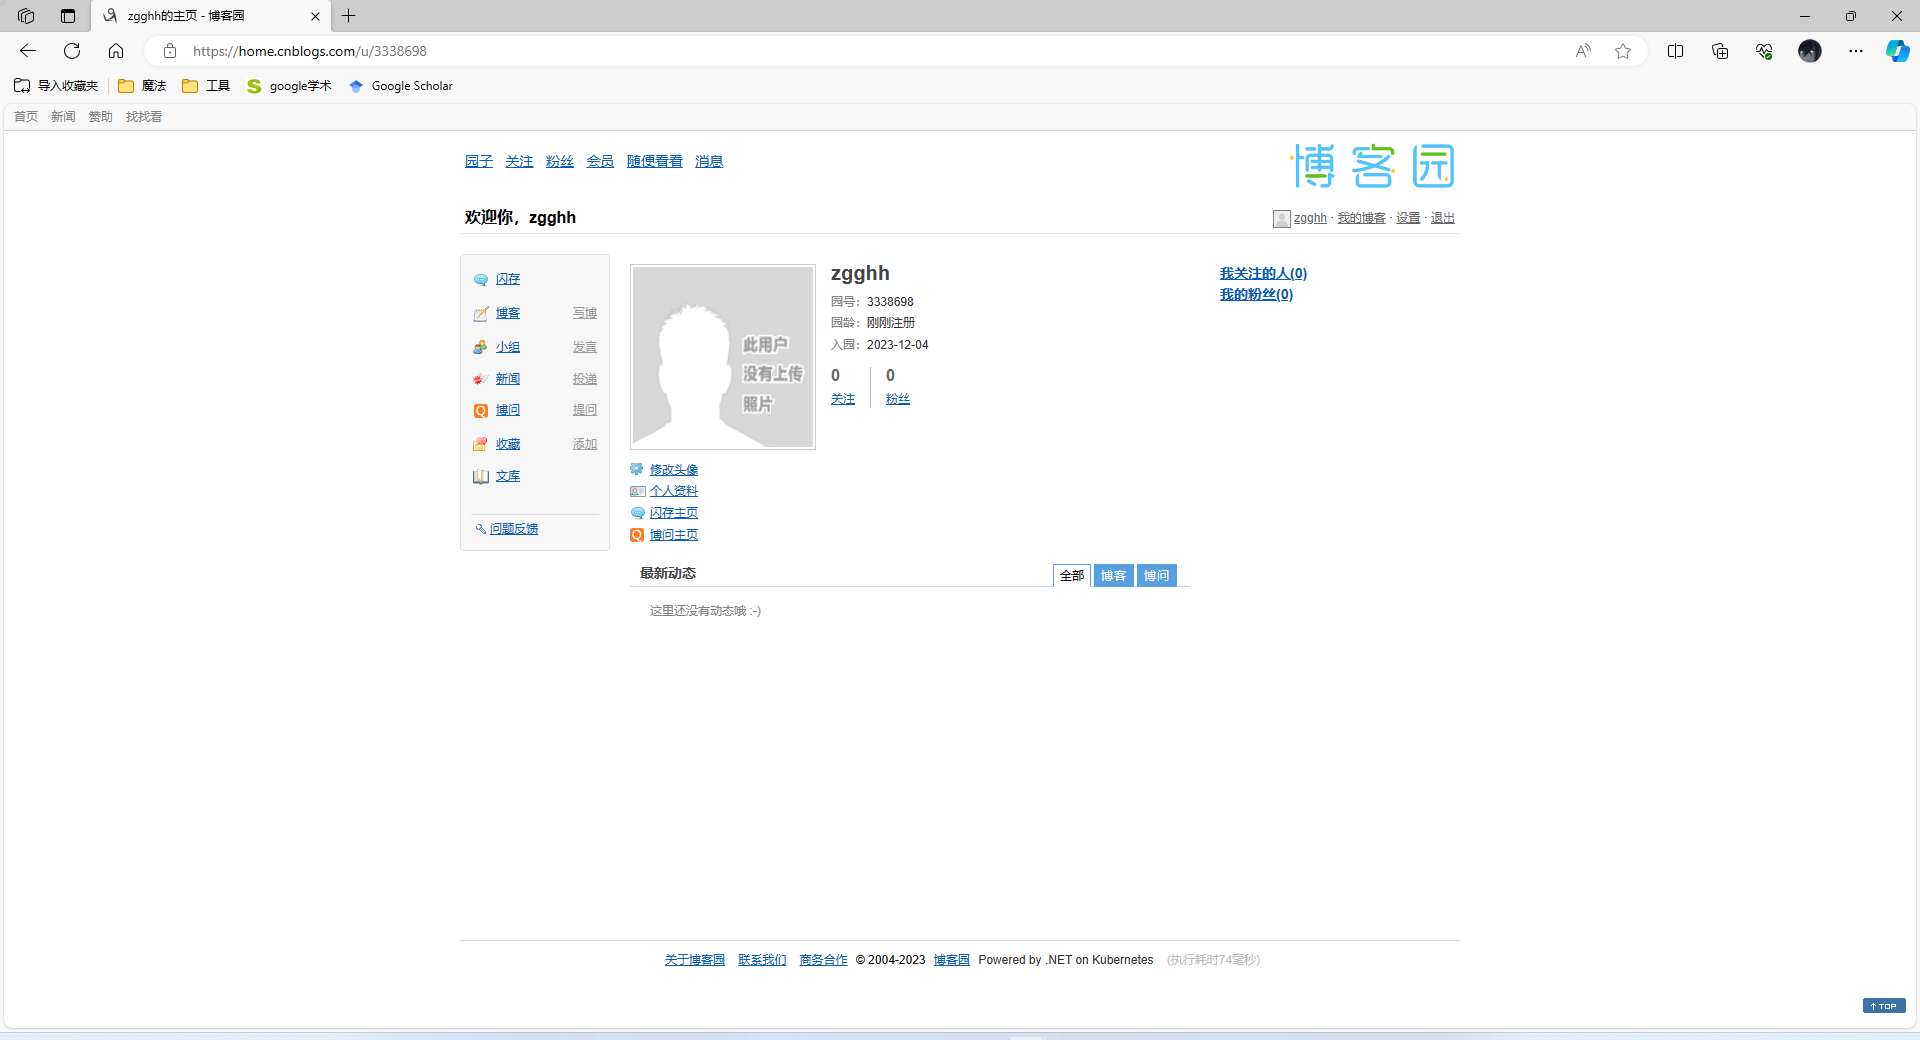
\includegraphics[width=9cm]{blog.png}
    	\caption{博客园个人网站截图}
    	\label{fig:blog}
    \end{figure}
    
    \item 小木虫
    
    注册小木虫账户,给出个人网址和个人网站截图\par
    http://muchong.com/bbs/space.php?uid=34311894
    \begin{figure}[h!]
    	\centering
    	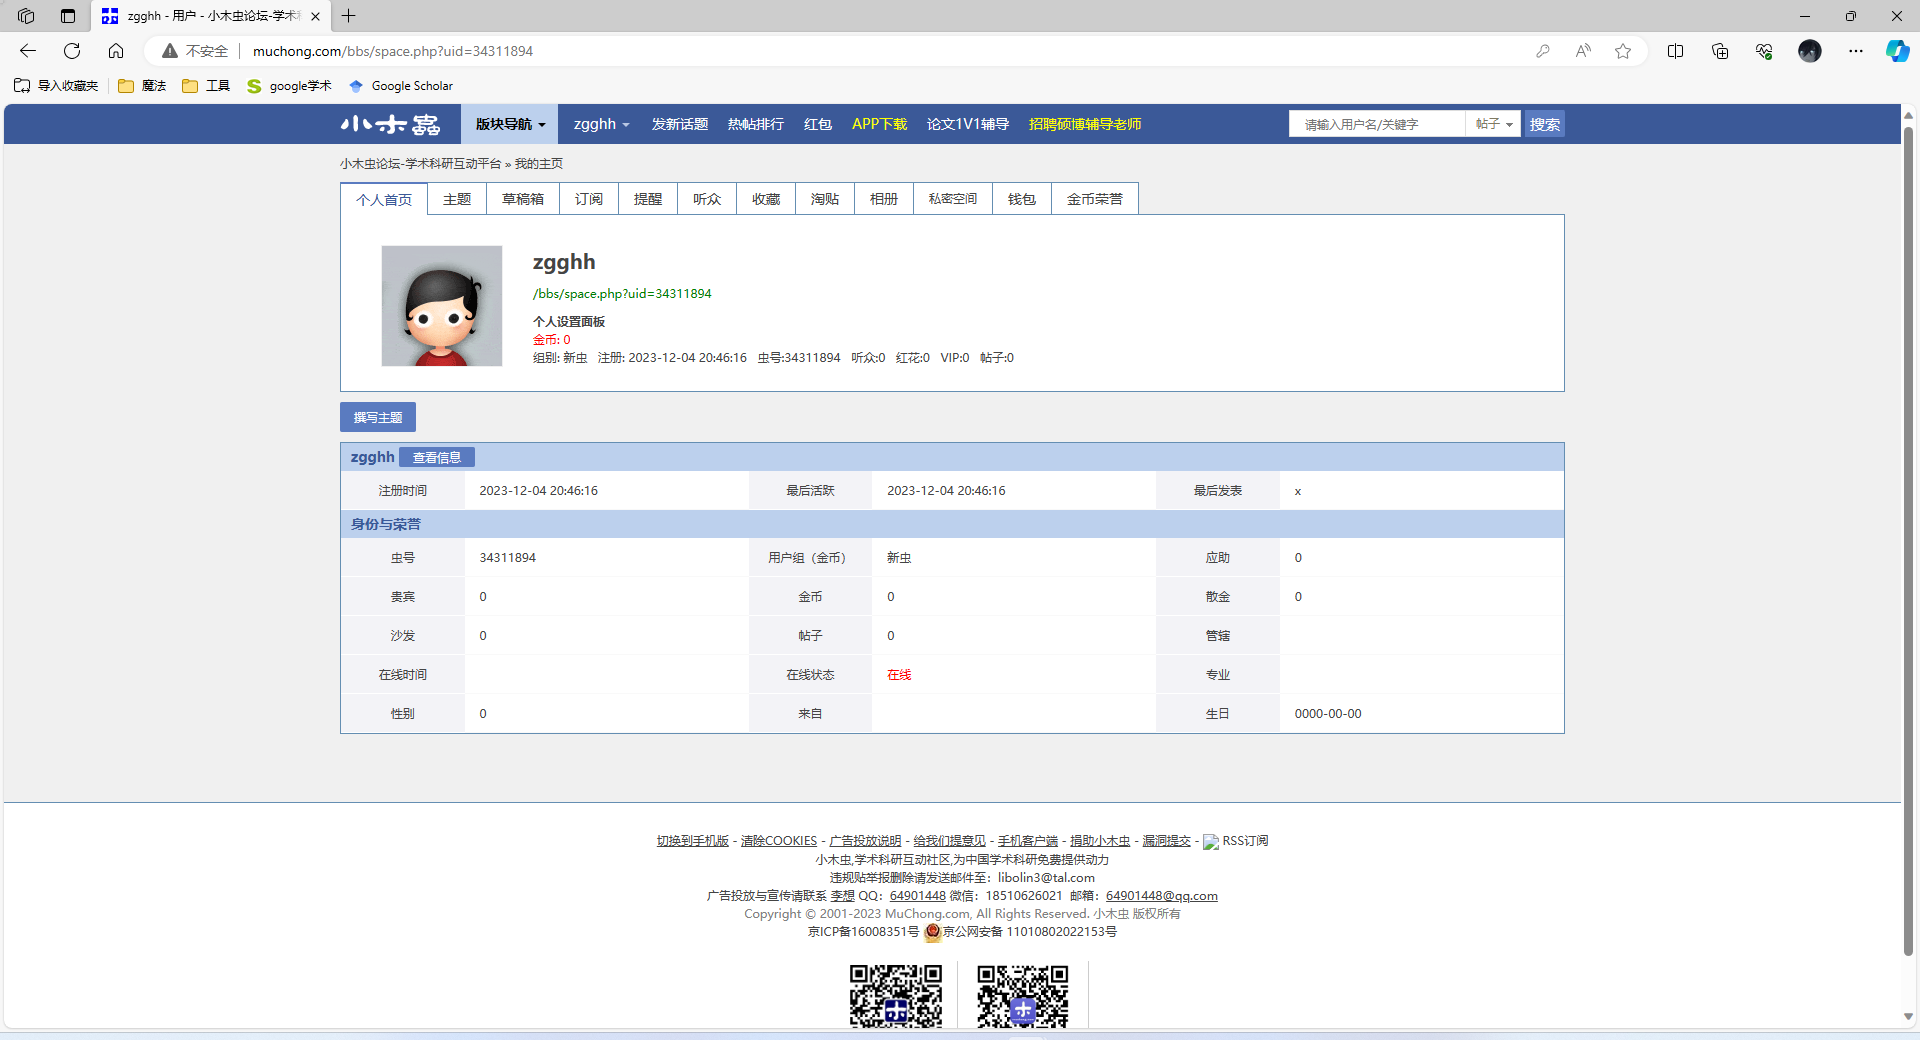
\includegraphics[width=9cm]{muchong.png}
    	\caption{小木虫个人网站截图}
    	\label{fig:muchong}
    \end{figure}
    
    
\end{itemize}


\hspace*{\fill} \\

%{\bf 注意,参考文献至少五篇,其中至少两篇为英文文献,参考文献必须在正文中有引用。}
%\bibliographystyle{plain}
%\bibliography{references}
\begin{thebibliography}{99}  
	
	\bibitem{ref1}Eden, A.H. Three Paradigms of Computer Science. Minds \& Machines 17, 135–167 (2007). https://doi.org/10.1007/s11023-007-9060-8
	\bibitem{ref2}Marc P. Armstrong (2000) Geography and Computational Science, Annals of the Association of American Geographers, 90:1, 146-156, DOI: 10.1111/0004-5608.00190
	\bibitem{ref3}LeCun Y, Bengio Y, Hinton G. Deep learning[J]. nature, 2015, 521(7553): 436-444.
	\bibitem{ref4}Turing, A.M.: Computing machinery and intelligence. Mind. 49, 433–460 (1950)
	\bibitem{ref5}Smullyan R M. Gödel's incompleteness theorems[M]. Oxford University Press, USA, 1992.
	
\end{thebibliography}


\end{document}
